%%%%%% CMB-S4 Simulations and Data Analysis Chapter, Time-Ordered Data Procesing Section  %%%%%%%%%%%%%%%%
 
\section{Time-Ordered Data Processing}

\subsection{Overview}

The time-ordered data processing elements of the CMB simulation and analysis pipeline -- simulation, pre-processing and mission characterization, and map-making -- are grouped as a subset due to the unique computational challenges posed by the volume of data that they must process.

\begin{figure}[htbp]
\centering
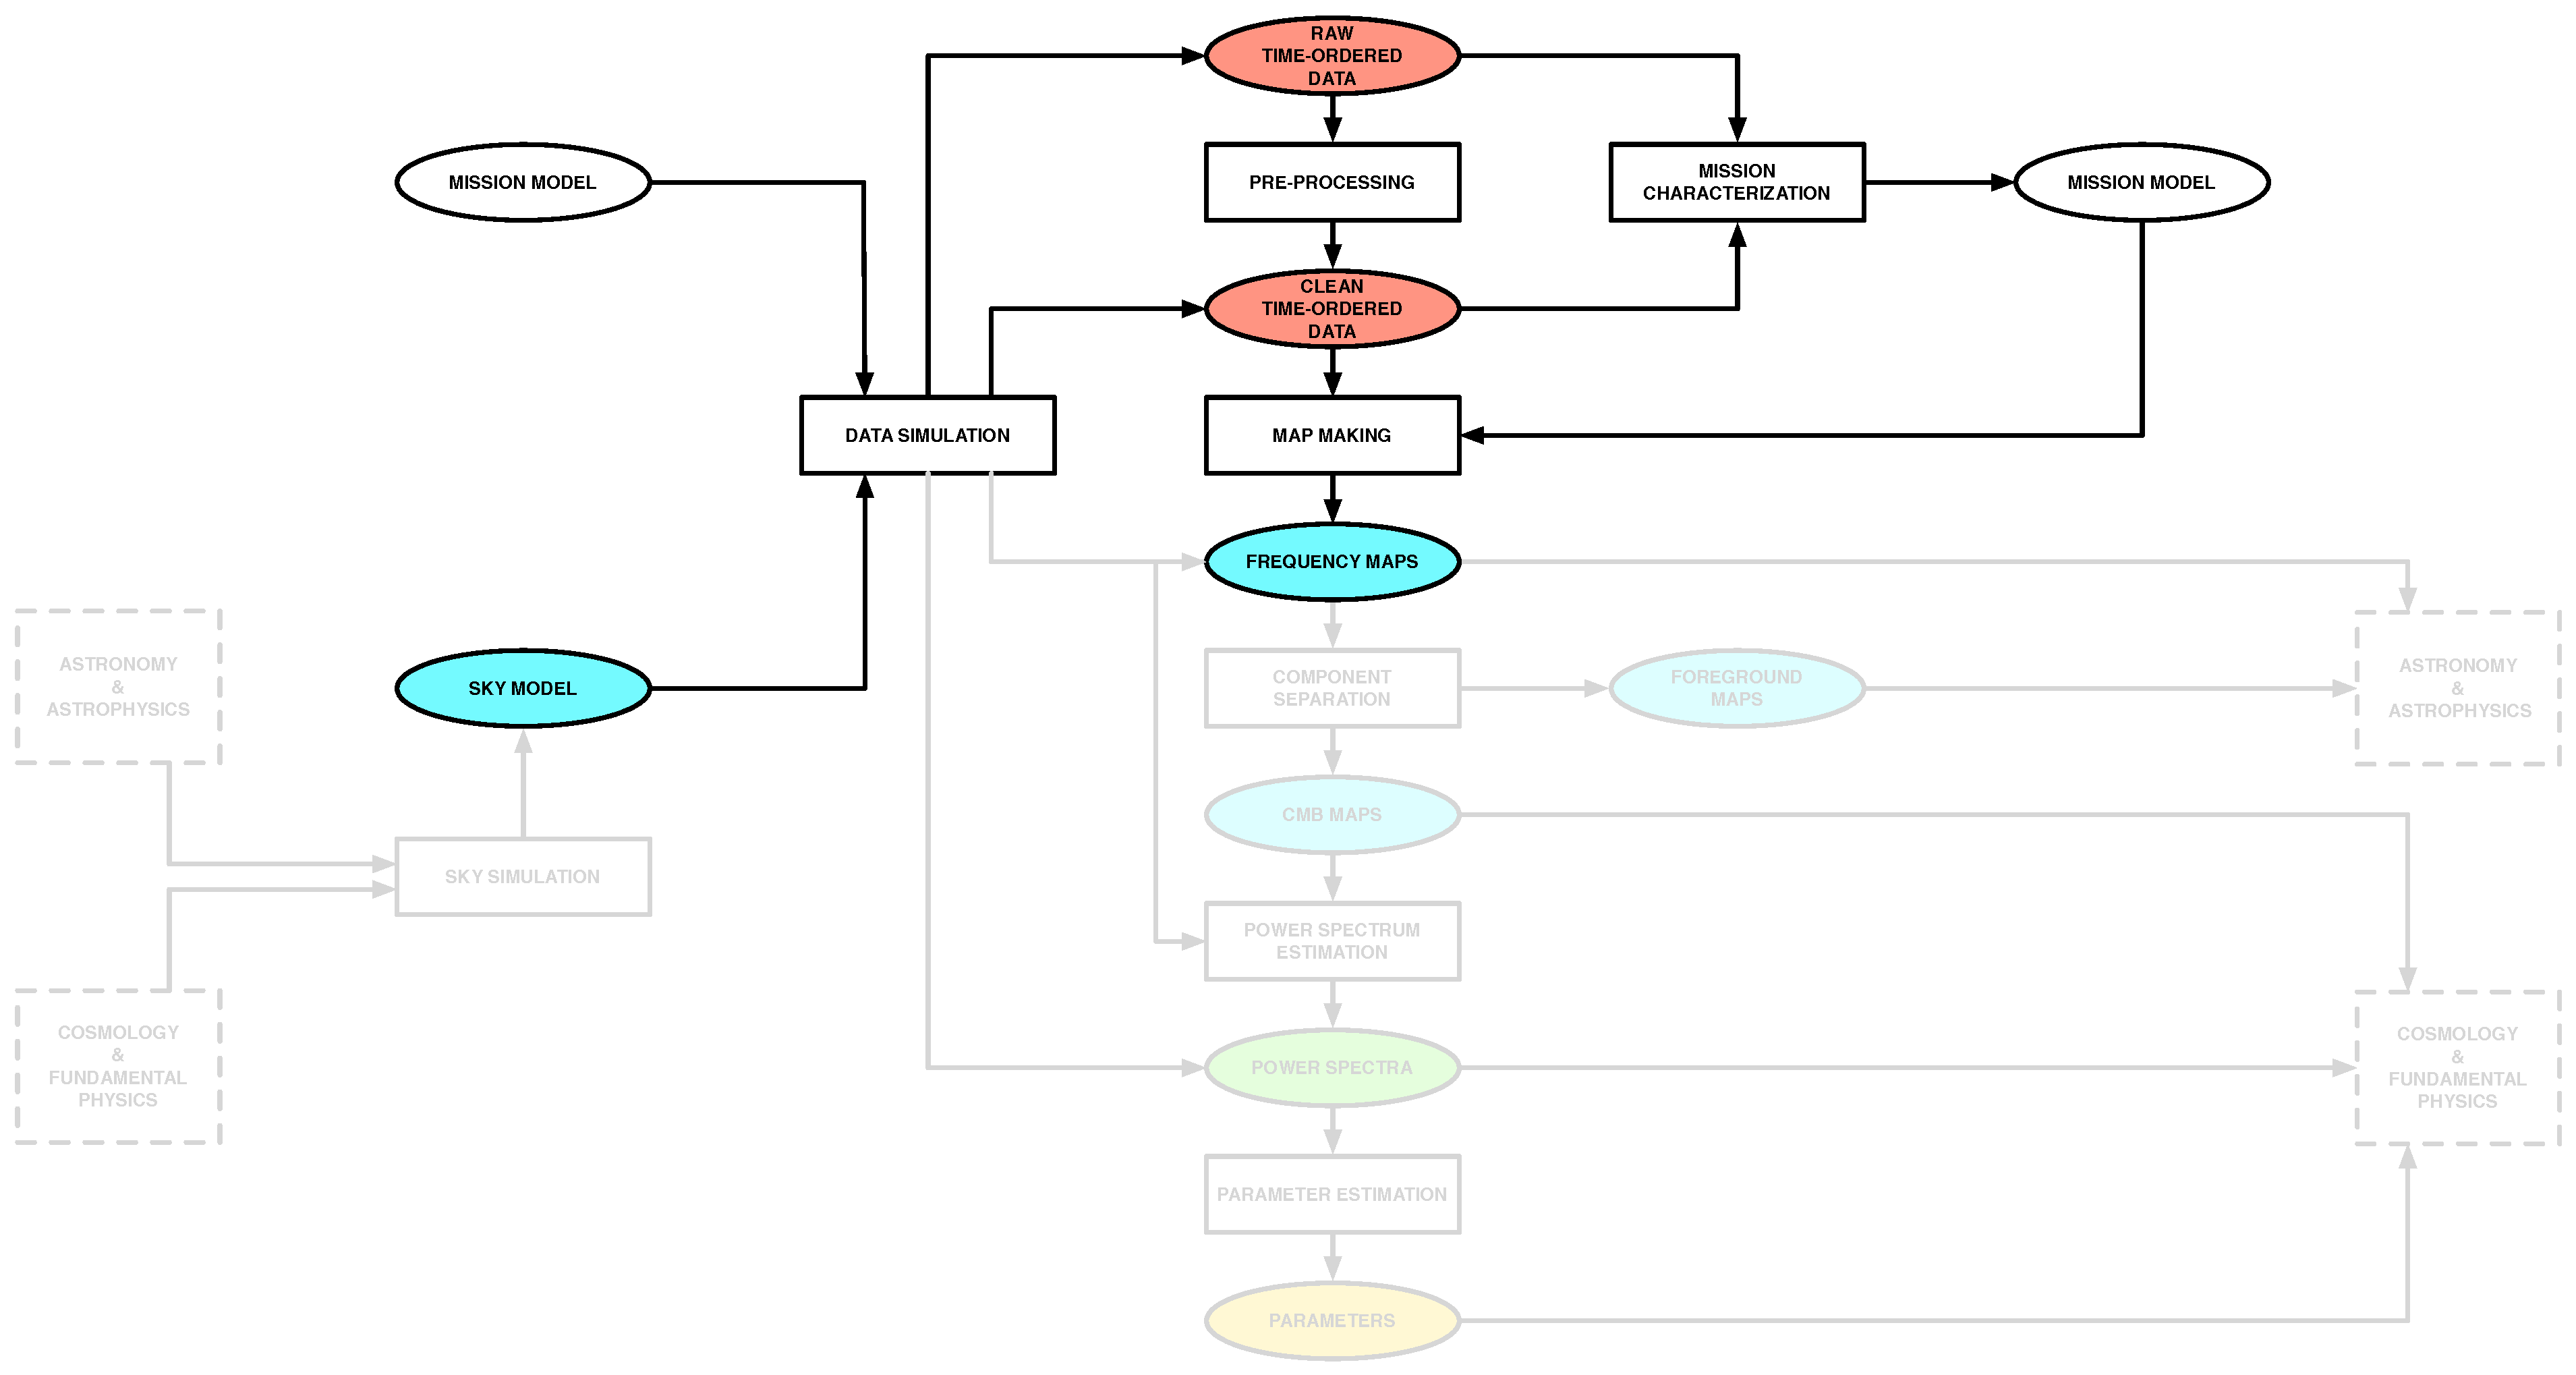
\includegraphics[width=1\textwidth]{Analysis/td}
\caption{The time-ordered data processing subset of the CMB simulation and data analysis pipeline}
\label{fig_td}
\end{figure}

\subsection{Simulation}

sky signal to instrument readout

instrument - beam, bandpass, noise; calibration, electronics

observation -- pointing, polarization (hwp), flagging, atmosphere

V \& V for other TOD processing elements

effective beam convolution

\subsection{Pre-Processing and Mission Characterization}

systematics mitigation: filtering, template-subtraction, marginalization

mission model building: pointing, beam, noise, systematics

\subsection{Map-Making}

Map-making is the stage of the data analysis when the major compression of the time domain ordered data happens and some estimate of the sky signal, typically in multiple frequency bands
is produced. Typically, map-making is considered to be a linear operation, characterized by some operator, $\mathbf{L}$, which transforms the input data, $\mathbf{d}$, into pixel domain object, $\mathbf{m}$, 
e.g., \cite{Tegmark1997},
\begin{eqnarray}
\mathbf{m} = \mathbf{L}\mathbf{d},
\end{eqnarray}
with a typical condition imposed on the the solution that the estimator is unbiased over the statistical ensemble of instrumental noise realizations, i.e.,
\begin{eqnarray}
\langle \mathbf{m} - \mathbf{s}\rangle = 0,
\label{eq:condMaps}
\end{eqnarray}
where $\mathbf{s}$ is the true, albeit pixelized, sky signal.
Given the standard model for the measurements, 
\begin{eqnarray}
\mathbf{d} = \mathbf{A}\mathbf{s} + \mathbf{n},
\end{eqnarray}
the condition leads to,
\begin{eqnarray}
\langle \mathbf{m} - \mathbf{s}\rangle =  (\mathbf{L}\mathbf{A}-\mathbf{1})\mathbf{s} 
+ \langle \mathbf{n} \rangle = (\mathbf{L}\mathbf{A}-\mathbf{1})\mathbf{s},
\end{eqnarray}
as the average noise is assumed to vanish. Hence,
\begin{eqnarray}
\mathbf{L}\mathbf{A} = \mathbf{1},
\end{eqnarray}
what  is solved by,
\begin{eqnarray}
\mathbf{L} = (\mathbf{A}^{\rm T} \mathbf{W} \mathbf{A})^{-1} \mathbf{A}^{\rm T} \mathbf{W}.
\end{eqnarray}
Here matrix $\mathbf{W}$ stands for an arbitrary, positive definite weight matrix. Different choices of the weights
lead to different sky signal estimates:
\begin{itemize}
\item if $\mathbf{W}$ is
fixed to correspond to the inverse of the true time domain noise, i.e., $\mathbf{W} = \mathbf{N}^{-1}$,
the sky signal estimate, $\mathbf{m}$, will correspond to the {\bf maximum likelihood} and {\bf minimum variance}
solutions. 
\item if instead the weights are taken to be proportional to some diagonal matrix minus some low-rank correction,
i.e., $\mathbf{W} \propto \mathbf{1} - \mathbf{T}\mathbf{T}^{\rm T}$,  where $\mathbf{T}$ s assumed to be column-orthogonal and the modes defined by its columns of 
are thus effectively removed (marginalized over)
from the solution. This approach incorporates as a special case so-called {\bf destriping approaches}, e.g.,~\cite{Poutanen2004, Keihanen2004}, which have gained
recently recognition thanks to their successful applications to the Planck data, e.g.,~\cite{Keihanen2010, Tristram2011, LFIMaps2015, HFImaps2015}, and are therefore of potential
interest for any 
experiments aiming at covering large swaths of the sky.
More generally, however matrix $\mathbf{T}$ can be tweaked to permit removal of unwanted, contaminated modes, e.g., 
due to the ground pick up, present in the time domain data, e.g.,~\cite{Stompor2001, Cantalupo2010, Dunner2013}.
\item if the weight matrix is taken to be diagonal, then the map-making solution corresponds to weighted co-addition
({\bf binning}) of samples in every sky pixel.
\end{itemize}
If the experimental beams display a complex, non-axially symmetric structure, proper estimation of the sky signal
may require correcting for these effects already on the map level leading to the so-called {\bf deconvolution algorithms}~\cite{ArmitageWandelt2004, Harrison2011, KeihanenReinecke2012}.  Further work is
however needed to demonstrate such approaches in more general cases.

If the map-making stage is performed mostly as a data compression operation on the way to derive some constraints
on statistical properties of the sky signal, such as its power spectra, one may opt for relaxing the condition in Eq.~(\ref{eq:condMaps})
in favor of quick to compute, albeit potentially biased sky estimate,
\begin{eqnarray}
\mathbf{m} = (\mathbf{A}^{\rm T} {\rm diag}( \mathbf{W}) \mathbf{A})^{-1} \mathbf{A}^{\rm T}\mathbf{W} \mathbf{d},
\end{eqnarray}
where ${\rm diag}( \mathbf{W})$ denotes a diagonal part of matrix $\mathbf{W}$.
In this approach the bias, if present, is then corrected on the next level of the data processing, e.g.,~\cite{Hivon2002}. This approach has been
proven to be not only computationally effective but also very efficient at least in the context of the experiments with a 
small sky coverage, e.g., \cite{QUAD2010, SPT2011, POLARBEAR, BICEP2014}.

The linearity of the mapmaking operation permits propagation of the uncertainty due to the instrumental noise from time domain level
to that of the maps,
\begin{eqnarray}
{\cal N} = \mathbf{L} \mathbf{N} \mathbf{L}^{\rm T},
\end{eqnarray}
this leads to a particularly simple expression for the maximum likelihood estimators yielding,
\begin{eqnarray}
{\cal N} = (\mathbf{A}^{\rm T} \mathbf{N}^{-1} \mathbf{A})^{-1}.
\end{eqnarray}
Though mathematically simple, due its sizes and numerical cost involved in its computations, such pixel-domain noise correlations
are rarely computed explicitly for the modern data sets and the uncertainty is either carried over to the next stages of the data processing 
in an implicit form or the final uncertainty computed with
help of the Monte Carlo simulations.

\subsection{Computational Constraints}



The computational requirements here are for both capacity and capability. To support the iterative exploration of the time-ordered data required by the pre-processing and mission characterization steps we need many analysts to be able to process the full data simultaneously, with each seeing no worse than order 1-day turnaround time for their jobs to complete. Conversely, to support the massive Monte Carlo simulation and map-making required for percent level uncertainty quantification in the absence of a full data covariance matrix, we need to be able to perform occasional runs of up to $10^4$ realizations within the total cycles available to us.

\begin{figure}[htbp]
\centering
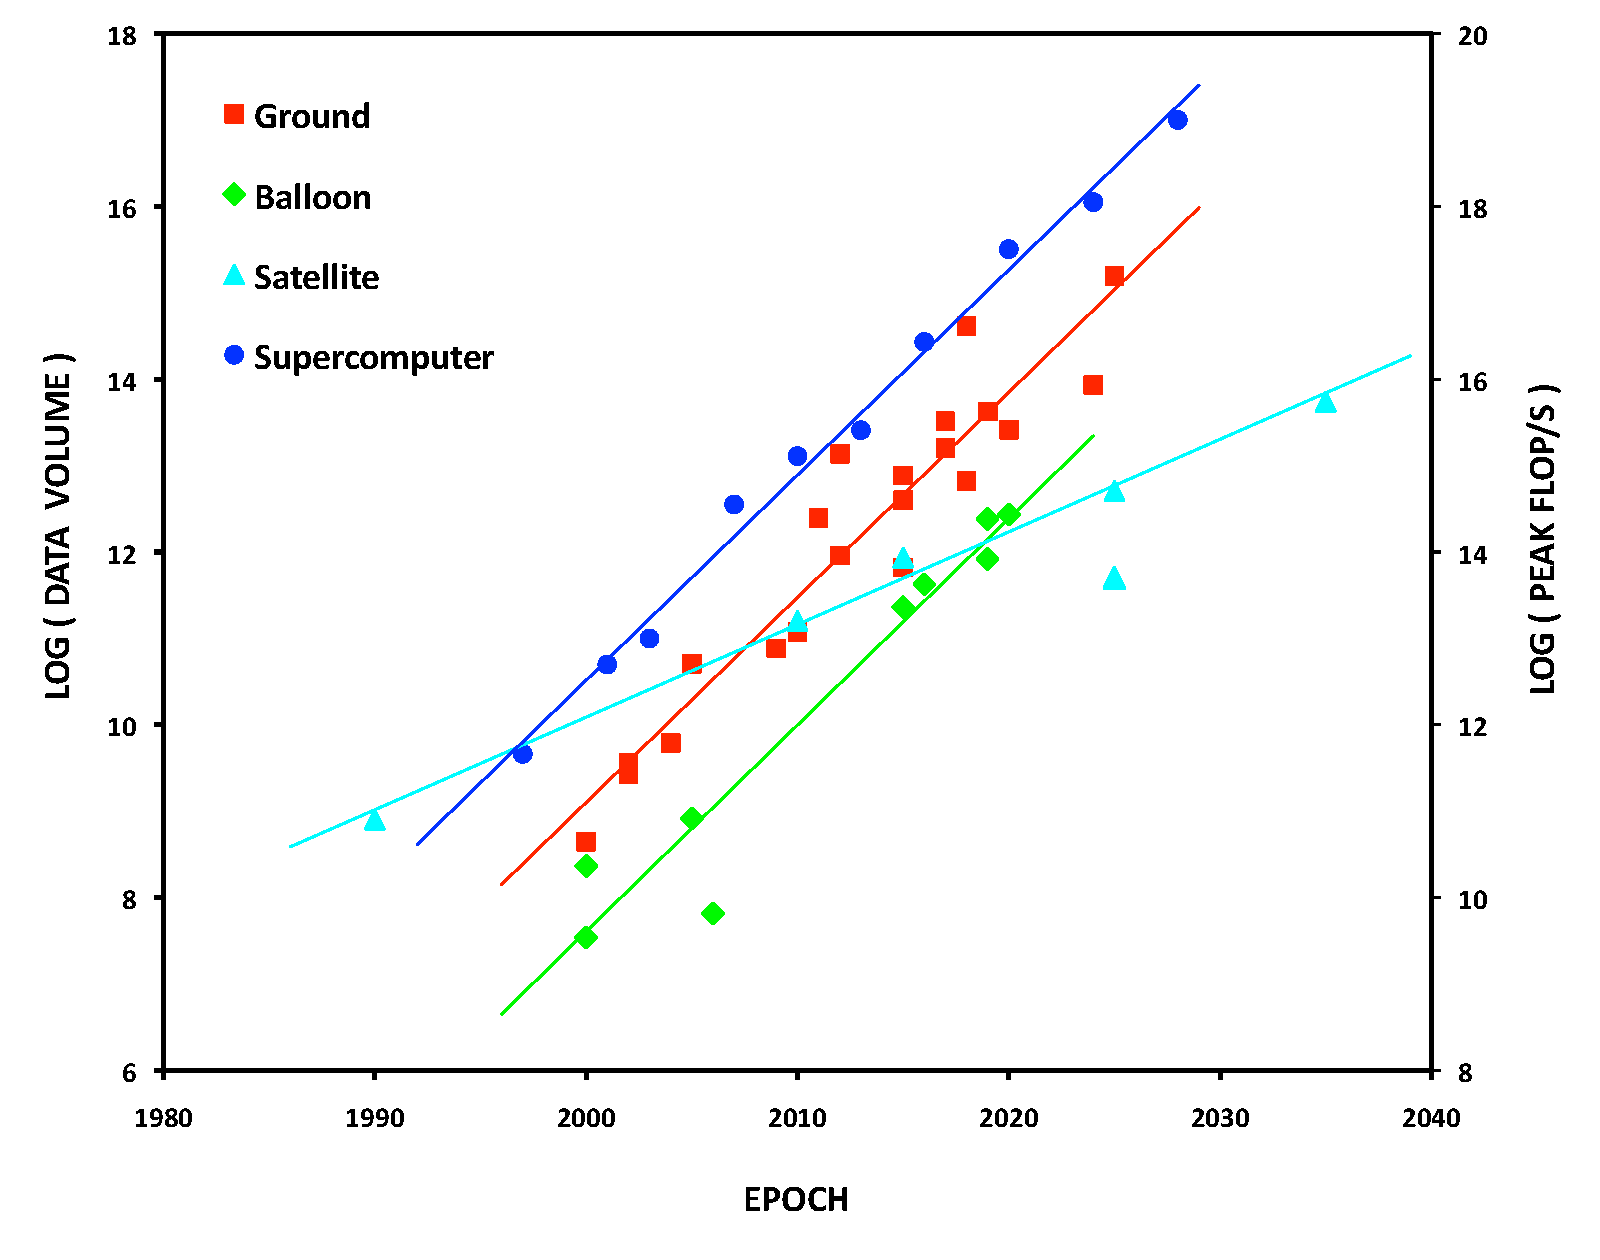
\includegraphics[width=0.5\textwidth]{Analysis/cmb_hpc_scaling}
\caption{Exponential growth of CMB time-ordered data volume and HPC capability: 1990 -- 2030.}
\label{fig_cmb_hpc_scaling}
\end{figure}

As Figure \ref{fig_cmb_hpc_scaling} shows, the size of ground-based, balloon-borne and satellite CMB data sets exhibit exponential growth over a 40 year period. Moreover, for suborbital experiments the exponent exactly matches that of Moore's Law, where we us as a proxy the peak performance of the flagship high performance computing (HPC) system at the DOE's National Energy Research Scientific Computing (NERSC) Center at any epoch (this choice reflecting the widespread use of NERSC for CMB data analyses over the last 20 years). 

As noted above, the intractability of pixel-domain data covariance matrices pushes us to use Monte Carlo (MC) methods for uncertainty quantification and debiasing, and the computational cost of the data analysis is dominated by the generation and reduction of sufficient MC realizations of the data for the resulting statistical error to be subdominant (typically assumed to be $10^4$ realizations for percent level uncertainty). 

Key challenges:
\begin{itemize}
\item computational tractability due to data volume and complexity of next-generation supercomputers
\item mitigating raw data systematics and developing sufficient mission and data models
\end{itemize}

All algorithmic and implementation choices we make must first and foremost be informed by their impact on computational tractability.

%\bibliography{cmbs4}

%%
%% Populate the .bib file with entries from SPIRES Bibtex (preferred)
%% or ADS Bibtex (if no SPIRES entry).
%%  SPIRES will also supply the CITATION line information; please include it.
%%


